     \chapter{Stuff you want to include}

A 1\degree C step input (\SI{35}{\milli\volt}), as shown in figure \ref{fig:ts}, was used to determine the settling time. The settling time is measured at the point where the output steps to 90\% of the final value (\SI{622}{\milli\volt}), which is \SI{560}{\milli\volt}. The settling time was thus measured as \SI{62.07}{ms}, as shown by the cursor difference in figure \ref{ts}.
\begin{figure}[h]
    \centering
    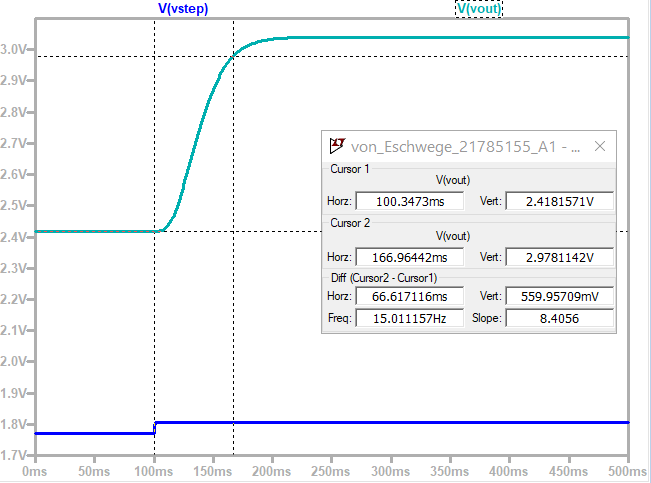
\includegraphics[width = 0.8\textwidth]{Figures/ts.png}
    \caption{Settling Time Measurement}
    \label{fig:ts}
\end{figure}

The bode plot for the low-pass filter is shown in figure \ref{fig:ac}. The -3dB point is lower than calculated, but is still well within the acceptable range. 
\begin{figure}[h]
    \centering
    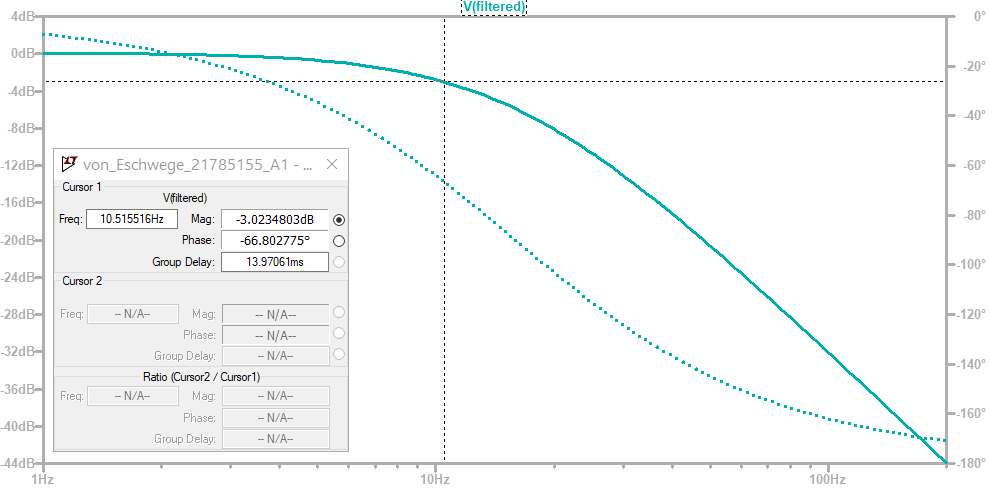
\includegraphics[width = 0.8\textwidth]{Figures/ac.png}
    \caption{Cutoff Frequency Measurement}
    \label{fig:ac}
\end{figure}

Please note:
It is a good design practice to include a unity gain op-amp to acts as a voltage buffer by clamping $V_{in-}$ against fluctuations. This design practice was considered, but ultimately rejected, as tests with and without the buffer provided outputs of equal quality. This is the case as the signal conditioning circuit already has a very high input resistance. The only notable differences resulting from the inclusion of a buffer were an increase in current drawn, as well as an increase in cost for the circuit components, as another op-amp is required. Therefore, in order to keep the current consumption below \SI{15}{mA}, as well as to use reduce cost by only using three op-amps, the voltage buffer was omitted in the final design.\\